\documentclass[UTF8,a4paper]{ctexart}
\usepackage{xcolor}
\usepackage{graphicx}
\usepackage[margin=1.5in]{geometry}
\usepackage{float}
\usepackage{listings} 
\usepackage{fancyhdr} %用于调整页眉的样式
\usepackage{fancyvrb} 
\usepackage{tabularx}
\usepackage[colorlinks,linkcolor=blue]{hyperref}%用于插入超链接
\usepackage{wallpaper}
\usepackage{tikz}
\usepackage{lipsum}
\usepackage{rotating}
\usepackage{multirow}
\usepackage[absolute]{textpos}
\usetikzlibrary{calc}
\setlength{\TPHorizModule}{1cm}
\setlength{\TPVertModule}{1cm}



\definecolor{color1}{RGB}{10,80,179}
\pagestyle{fancy}
\fancyhead[L]{\url{https://github.com/eric041224/tool_class_2024_sum}}
\setlength{\headheight}{27pt}

\definecolor{GradientTop}{RGB}{0,0,255}
\definecolor{GradientBottom}{RGB}{255,0,0}
\colorlet{GradientMid}{blue!50!red}

\lstset{
    numbers=left,
    numberstyle=\tiny,
    frame=shadowbox,
    rulesepcolor= \color{ red!20!green!20!blue!20},
    escapeinside=``,
    xleftmargin=2em,aboveskip=1em,
    framexleftmargin=2em,
    breaklines=true
}

\hypersetup{
    colorlinks=true,            % 激活链接颜色,去掉链接边框
    urlcolor=color1           % 外部URL链接颜色
}

\begin{document}
%封面
\ThisCenterWallPaper{1.02}{background.png} 
\begin{textblock}{5}(1,2)
    % 设置字号为20pt
    \fontsize{15}{24}\selectfont
    \color{white}
    \begin{turn}{270}
         \qquad 取则行远
        \end{turn}
        \begin{turn}{270}
            海纳百川 
            \end{turn}
    
    \end{textblock}
\begin{center}
    %logo
    \begin{tikzpicture}[remember picture, overlay]
        % 绘制一个矩形,并设置其位置在页面的右上角
        \draw[fill=blue] (current page.north east) rectangle (current page.north west);
        % 在矩形中插入图片,并设置与右上角的距离
        \node[anchor=north east, xshift=-1cm, yshift=-2cm] at (current page.north east) {
            
\includegraphics[width=6cm]{logo.png}
        };
    \end{tikzpicture}

\begin{textblock}{5}(1,24)
    
    \fontsize{120}{24}\selectfont
    \color{color1}
    Week4
       
    
    \end{textblock}

\begin{textblock}{5}(14.5,24)
    
    \fontsize{19}{24}\selectfont
    \color{color1}
    \raggedleft
    左昊天\\
    2024-09-13 \\
    \href{https://github.com/eric041224/tool_class_2024_sum}{Github 仓库地址}\\ 
    
    \end{textblock}

   
\end{center}

\thispagestyle{empty}

\newpage
\color{black}
\section{调试与性能分析}
\subsection{打印颜色}
\begin{lstlisting}
#!/usr/bin/env bash
for R in $(seq 0 20 255); do
    for G in $(seq 0 20 255); do
        for B in $(seq 0 20 255); do
            printf "\e[38;2;${R};${G};${B}m█\e[0m";
        done
    done
done
\end{lstlisting}
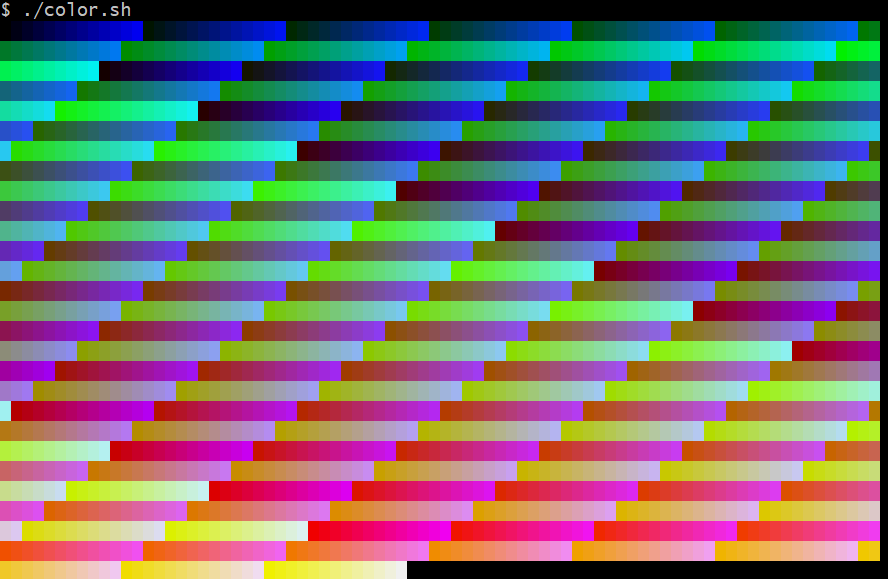
\includegraphics[width=1\textwidth]{./pictures/color.png}

\subsection{使用 Linux 上的 journalctl 或 macOS 上的 log show 命令来获取最近一天中超级用户的登录信息及其所执行的指令。如果找不到相关信息,您可以执行一些无害的命令,例如 sudo ls 然后再次查看。}
\begin{table}[H]
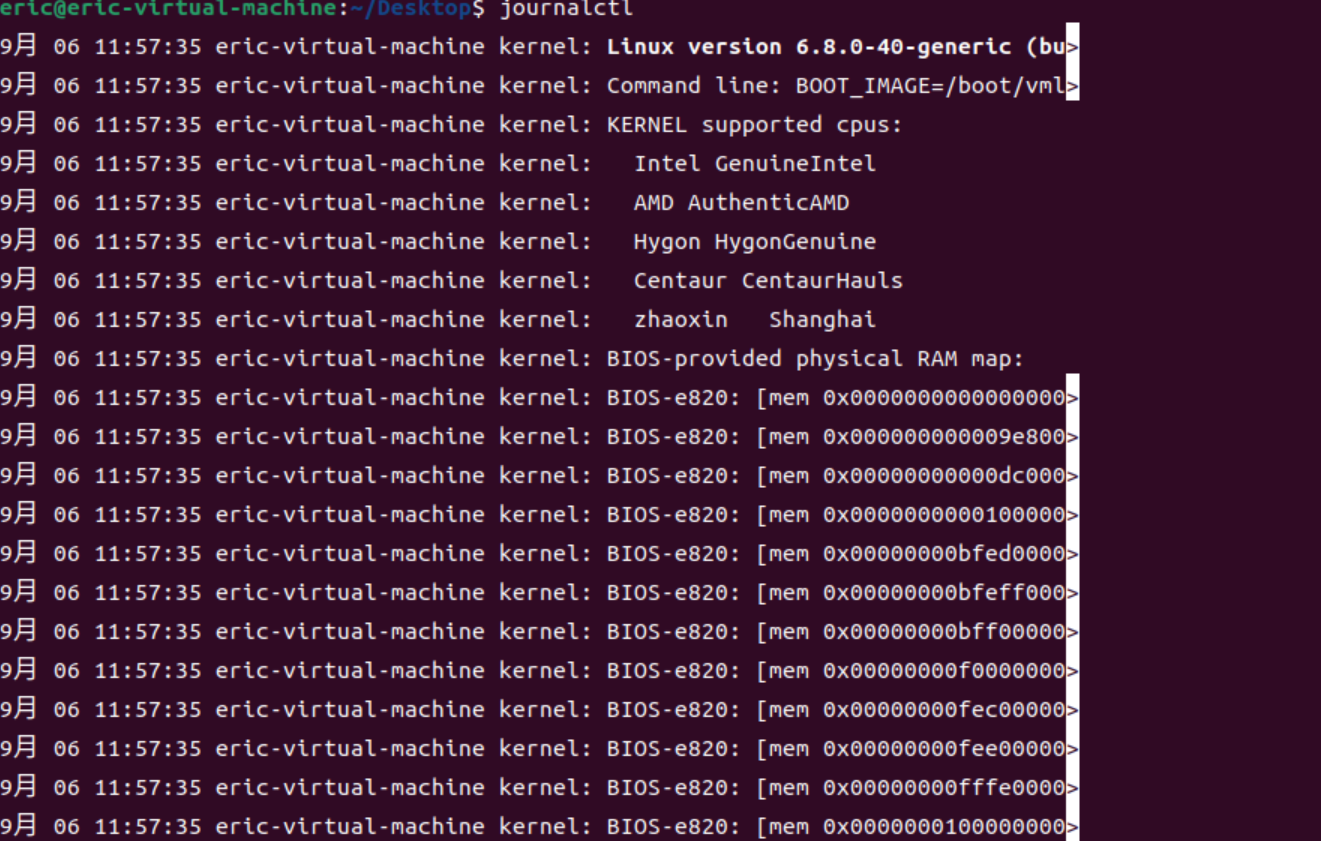
\includegraphics[width=1\textwidth]{./pictures/log.png}
\end{table}
\subsection{pdb调试器}
l(ist) - 显示当前行附近的 11 行或继续执行之前的显示;\par
s(tep) - 执行当前行,并在第一个可能的地方停止;\par
n(ext) - 继续执行直到当前函数的下一条语句或者 return 语句;\par
b(reak) - 设置断点(基于传入的参数);\par
p(rint) - 在当前上下文对表达式求值并打印结果。还有一个命令是 pp ,它使用 pprint 打印;\par
r(eturn) - 继续执行直到当前函数返回;\par
q(uit) - 退出调试器。\\
\textbf{这里使用的是ipdb,它是pdb的增强版本,相较于pdb有直观的界面显示。}\\
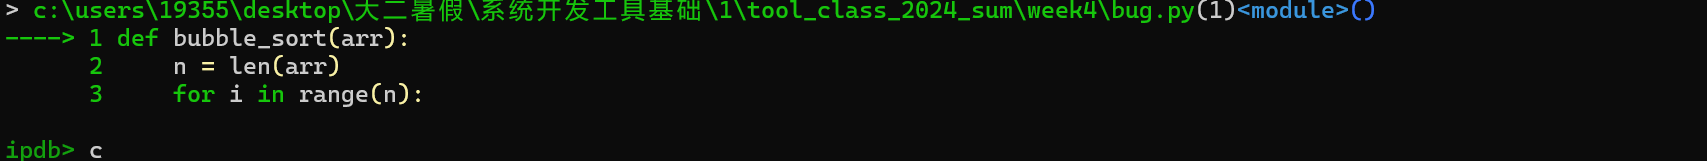
\includegraphics[width=1\textwidth]{./pictures/bug1.png}
c命令代表继续执行,直到出现错误。\\
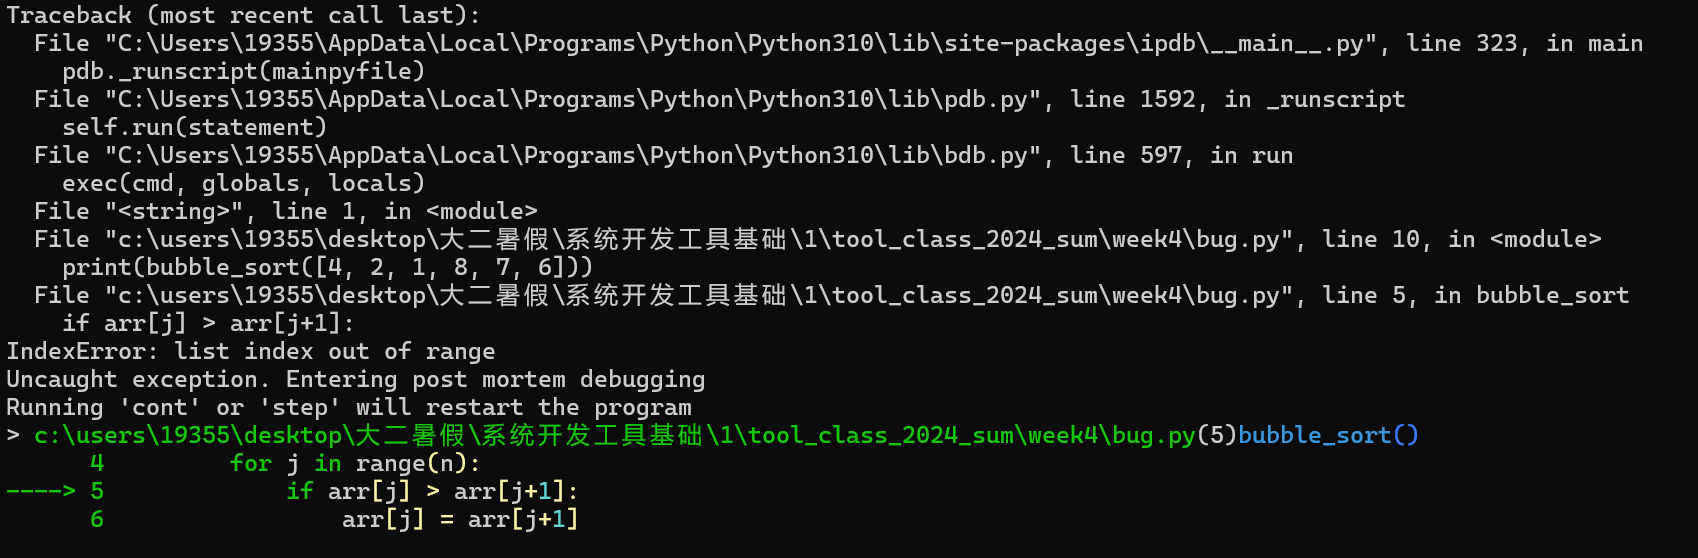
\includegraphics[width=1\textwidth]{./pictures/bug2.png}
使用p locals()命令,可以查看此时所有变量的值,用此进行错误分析。\\
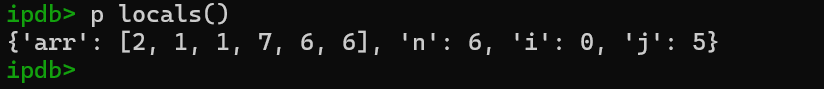
\includegraphics[width=1\textwidth]{./pictures/bug3.png}
\subsection{计时}
使用time库中的time函数
\begin{lstlisting}
import time, random
n = random.randint(1, 10) * 100

# 获取当前时间 
start = time.time()

# 执行一些操作
print("Sleeping for {} ms".format(n))
time.sleep(n/1000)

# 比较当前时间和起始时间
print(time.time() - start)

\end{lstlisting}
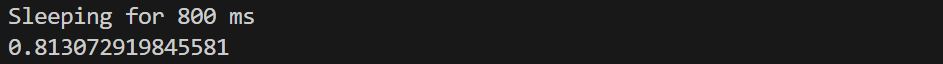
\includegraphics[width=1\textwidth]{./pictures/time.png}

\subsection{memory-profiler}
使用memory-profiler模块对内存进行监控。\\
实例代码:
\begin{lstlisting}
@profile
def my_func():
    a = [1] * (10 ** 6)
    b = [2] * (2 * 10 ** 7)
    del b
    return a

if __name__ == '__main__':
    my_func()
\end{lstlisting}
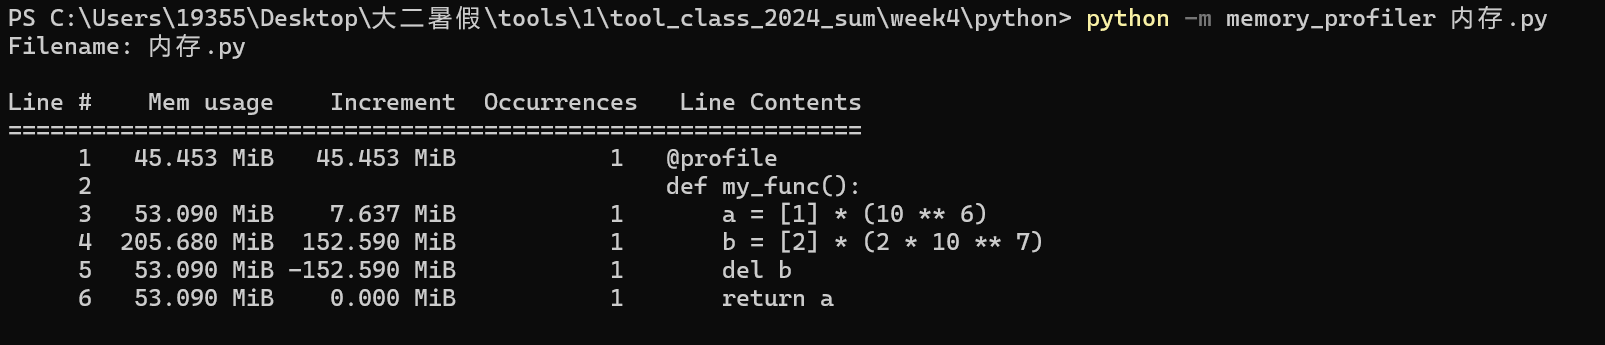
\includegraphics[width=1\textwidth]{./pictures/内存.png}

\subsection{shellcheck}
shellcheck是一个静态的脚本分析工具,它可以得到程序错误的原因。
\begin{lstlisting}
    shellcheck 文件名
\end{lstlisting}
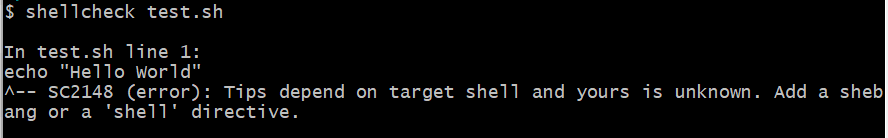
\includegraphics[width=1\textwidth]{./pictures/shellcheck1.png}
此代码的问题是开头没有声明使用的shell类型。需加上\verb|#!/bin/bash|

\subsection{这里有一些用于计算斐波那契数列 Python 代码,它为计算每个数字都定义了一个函数。将代码拷贝到文件中使其变为一个可执行的程序。首先安装 pycallgraph 和 graphviz(如果您能够执行 dot, 则说明已经安装了 GraphViz.)。并使用 pycallgraph graphviz -- ./fib.py 来执行代码并查看 pycallgraph.png 这个文件。fibN 被调用了多少次?我们可以通过记忆法来对其进行优化。将注释掉的部分放开,然后重新生成图片。这回每个 fibN 函数被调用了多少次?}
\begin{lstlisting}
#!/usr/bin/env python
def fib0(): return 0

def fib1(): return 1

s = """def fib{}(): return fib{}() + fib{}()"""

if __name__ == '__main__':

    for n in range(2, 10):
        exec(s.format(n, n-1, n-2))
    # from functools import lru_cache
    # for n in range(10):
    #     exec("fib{} = lru_cache(1)(fib{})".format(n, n))
    print(eval("fib9()")) 
\end{lstlisting}
\begin{figure}[H]
    \centering
    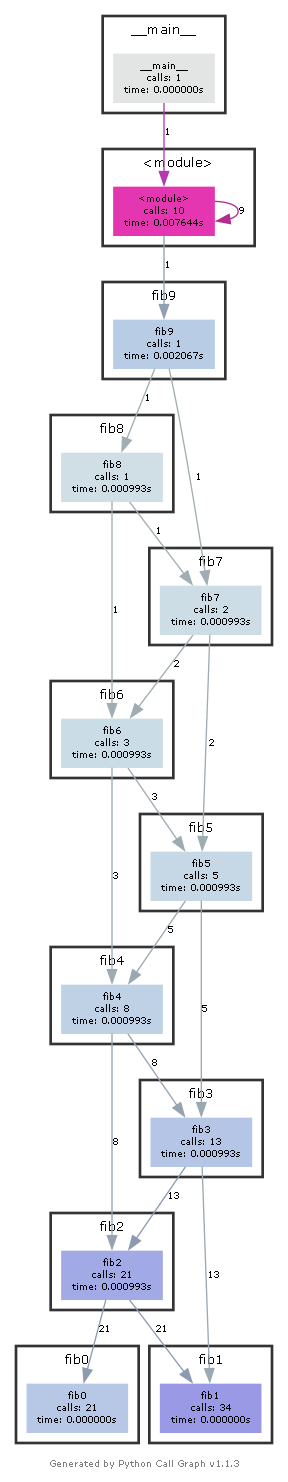
\includegraphics[width=0.3\textwidth]{./python/pycallgraph1.png}
    \caption{放开注释前}
    \textbf{\textcolor{color1}{被调用101次}}
\end{figure}
\begin{figure}[H]
    \centering
    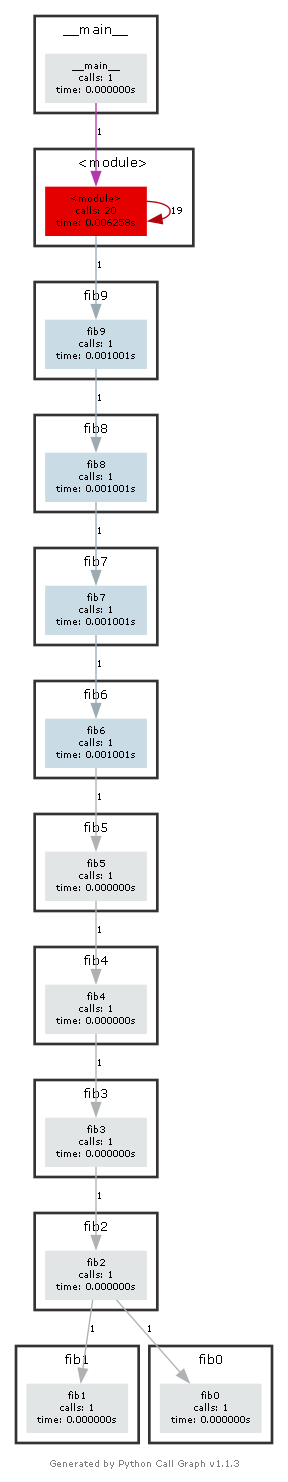
\includegraphics[width=0.3\textwidth]{./python/pycallgraph2.png}
    \caption{放开注释后}
    \textbf{\textcolor{color1}{被调用10次}}
\end{figure}


\subsection{遇到的问题:无法安装pycallgraph}
一开始根据提示,尝试回退setuptools版本,发现没有用。在网上不断搜索,找到解决方法,安装时用pip install pycallgraph2命令就可以安装了。

\section{元编程}
\subsection{makefile的写法}
\begin{lstlisting}
paper.pdf: paper.tex plot-data.png
pdflatex paper.tex

plot-%.png: %.dat plot.py
	plot.py -i $*.dat -o $@
\end{lstlisting}
冒号左侧的是构建目标,冒号右侧的是构建它所需的依赖。缩进的部分是构建时用到的命令

\subsection{生成图片的规则,和latex的写法}
\subsubsection{python(用于生成图片)}
\begin{lstlisting}
import matplotlib
import matplotlib.pyplot as plt
import numpy as np
import argparse

parser = argparse.ArgumentParser()
parser.add_argument('-i', type=argparse.FileType('r'))
parser.add_argument('-o')
args = parser.parse_args()

data = np.loadtxt(args.i)
plt.plot(data[:, 0], data[:, 1])
plt.savefig(args.o)
\end{lstlisting}
\subsubsection{latex(将生成的图片放入latex中)}
\begin{lstlisting}
\documentclass{article}
\usepackage{graphicx}
\begin{document}
\includegraphics[scale=0.65]{plot-data.png}
\end{document}
\end{lstlisting}
\subsubsection{.dat 数据文件}
\begin{lstlisting}
1 1
2 2
3 3
4 4
5 8
\end{lstlisting}
\subsection{make语句}
make后不加参数将会构建plot-data.png和paper.pdf文件;
但,如果make后加参数,比如make plot-data.png则只会构建这一个文件。
当然,只有在图片文件存在的情况下,才可以单独构建paper.pdf文件。
生成的图片:\\
\includegraphics[width=1\textwidth]{./makefile/plot-data.png}
latex生成的pdf:\\
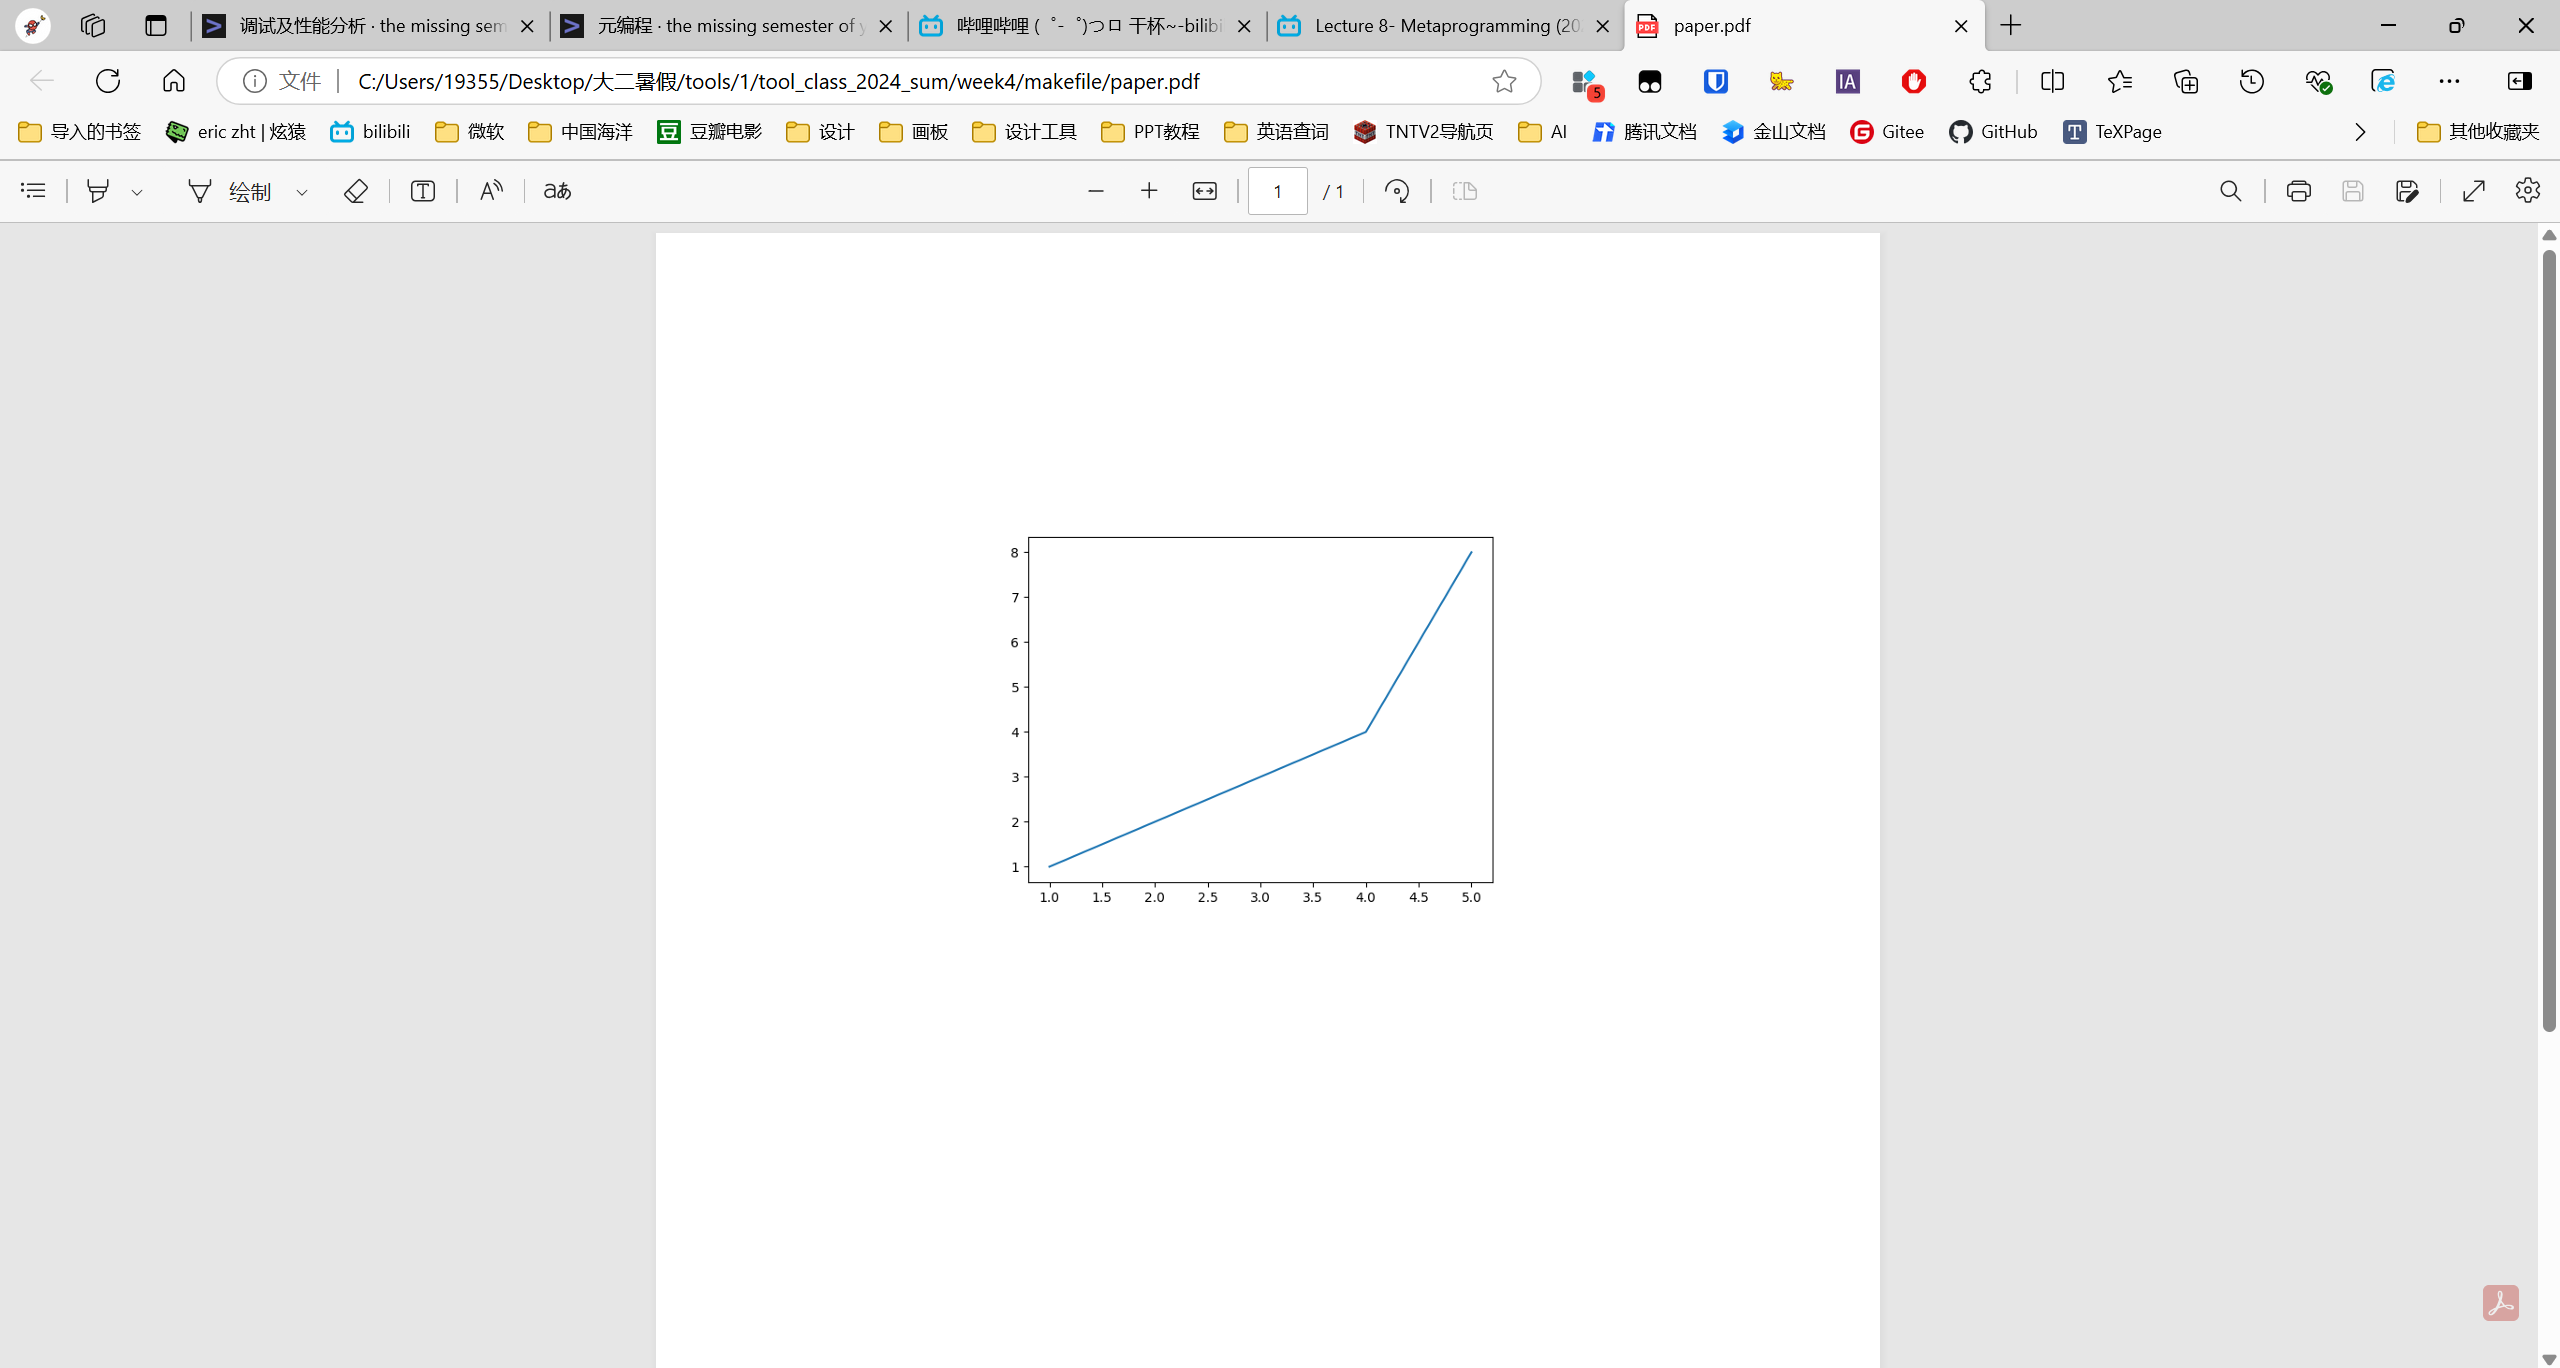
\includegraphics[width=1\textwidth]{./pictures/pdf.png}
\subsection{遇到的问题}
一开始一直报错,试了很多办法都没有解决。最开始使用的是windows shell,所以没有察觉出路径有什么问题
后来先去做别的,再返回来做这个时发现,在git bash中会出现无法显示的内容,考虑是中文引起的。将所有路径的中文改成英文后可以运行了。
同时makefile里其实是可以用相对路径的,但由于一开始使用的是绝对路径,才导致中文路径造成的影响。经测试,用相对路径时,路径中的中文不影响代码运行。\\
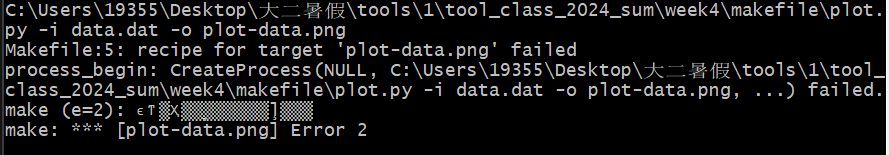
\includegraphics[width=1\textwidth]{./pictures/makefile1.png}

\subsection{大多数的 makefiles 都提供了 一个名为 clean 的构建目标,这并不是说我们会生成一个名为clean的文件,而是我们可以使用它清理文件,让 make 重新构建。您可以理解为它的作用是“撤销”所有构建步骤。在上面的 makefile 中为paper.pdf实现一个clean 目标。您需要构建phony。}
修改后的代码:
\begin{lstlisting}
paper.pdf: paper.tex plot-data.png
	pdflatex paper.tex

plot-%.png: %.dat plot.py
	./plot.py -i $*.dat -o $@

.PHONY: clean
clean:
	rm *.pdf *.aux *.log *.png    
\end{lstlisting}
当文件存在,并且数据没有任何更新时,输入make命令并不会重新构建文件。\\
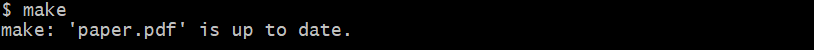
\includegraphics[width=1\textwidth]{./pictures/makefile3.png}
这时就体现\verb|.PHONY|的作用了,\verb|.PHONY|是用于声明伪目标的关键字。伪目标不是文件。
如果目标与实际文件同名,make 可能会认为目标是已经存在的,不需要重新执行。如果存在名为 clean 的文件,make clean 将不会执行 clean 目标,因为 make 认为 clean 已经是一个文件。使用 \verb|.PHONY: clean|,make 会忽略文件的存在,强制执行 clean 目标。
在这里make clean命令用于删除前面make构建的文件。\\
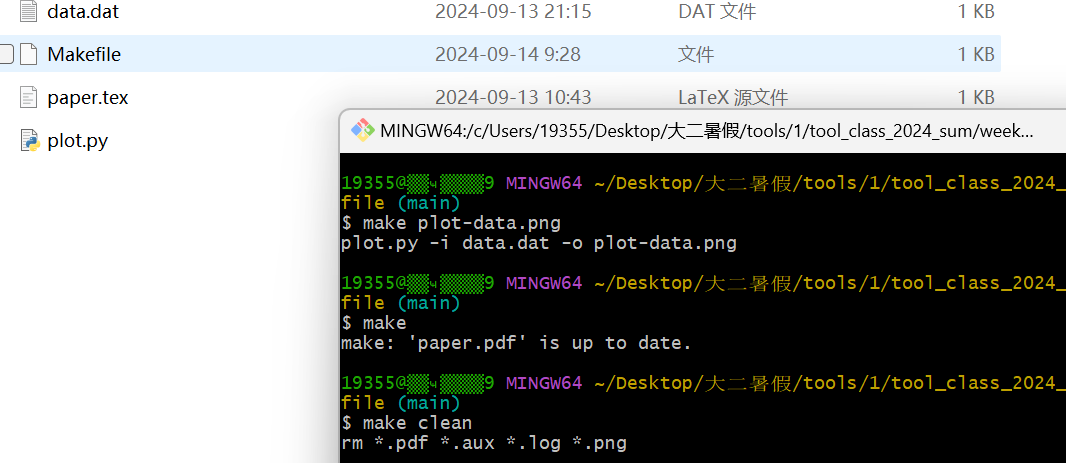
\includegraphics[width=1\textwidth]{./pictures/clean.png}

\subsection{版本号}
\textbf{主版本号.次版本号.补丁号}\\
关于版本号的规则:\\
如果新的版本没有改变 API,递增补丁号;\\
如果添加了 API 并且该改动是向后兼容的,递增次版本号;\\
如果修改了 API 但是它并不向后兼容,递增主版本号。\\



\section{pytorch}
\subsection{引入库}
\begin{lstlisting}
from __future__ import print_function
import torch
\end{lstlisting}
\textbf{注:以下代码均省略引入库的代码。}
\subsection{随机生成 a × b 的矩阵}
\begin{lstlisting}
rand_x = torch.rand(a, b)
print(rand_x)
\end{lstlisting}
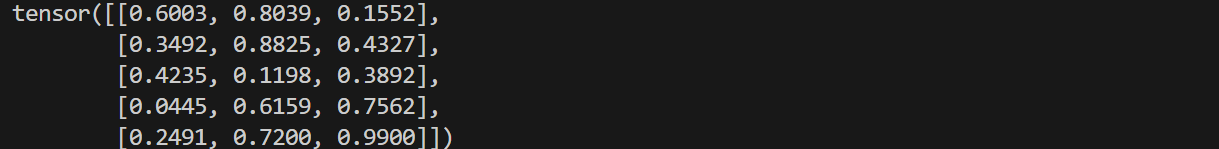
\includegraphics[width=1\textwidth]{./pictures/tensor1.png}
(此为5×3的矩阵)
\subsection{创建数值都是0,类型为long的矩阵}
\begin{lstlisting}
zero_x = torch.zeros(a, b, dtype=torch.long)
print(zero_x)
\end{lstlisting}
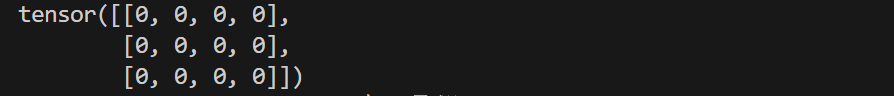
\includegraphics[width=1\textwidth]{./pictures/tensor2.png}
\subsection{保留相同的尺寸大小,并修改数据类型}
\begin{lstlisting}
tensor1 = torch.zeros(3, 4, dtype=torch.long)
tensor2 = torch.randn_like(tensor1, dtype=torch.float)
print('tensor1: ', tensor1)
print('tensor2: ', tensor2)
\end{lstlisting}
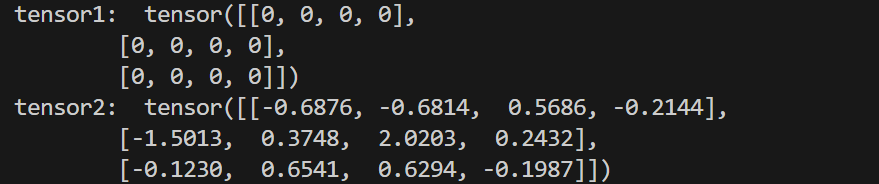
\includegraphics[width=1\textwidth]{./pictures/tensor3.png}
\subsection{修改tensor的尺寸}
\begin{lstlisting}
x = torch.randn(3, 6)
y = x.view(18)
# -1 表示除给定维度外的其余维度的乘积
z = x.view(-1, 9)
print(x.size(), y.size(), z.size())
\end{lstlisting}
解释:z矩阵的列计算方式:\\
x是4×4的,所以总共有18个。z的列乘以行数(9)等于18,所以z的列数为2。
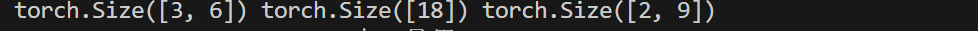
\includegraphics[width=1\textwidth]{./pictures/tensor4.png}

\subsection{Tensor 的加法}
三种方式:\par
1、\verb|+|\par
2、\verb|torch.add(tensor1, tensor2)|\par
3、\verb|tensor1.add_(tensor2)|,该方法会直接修改tensor1变量的值\\
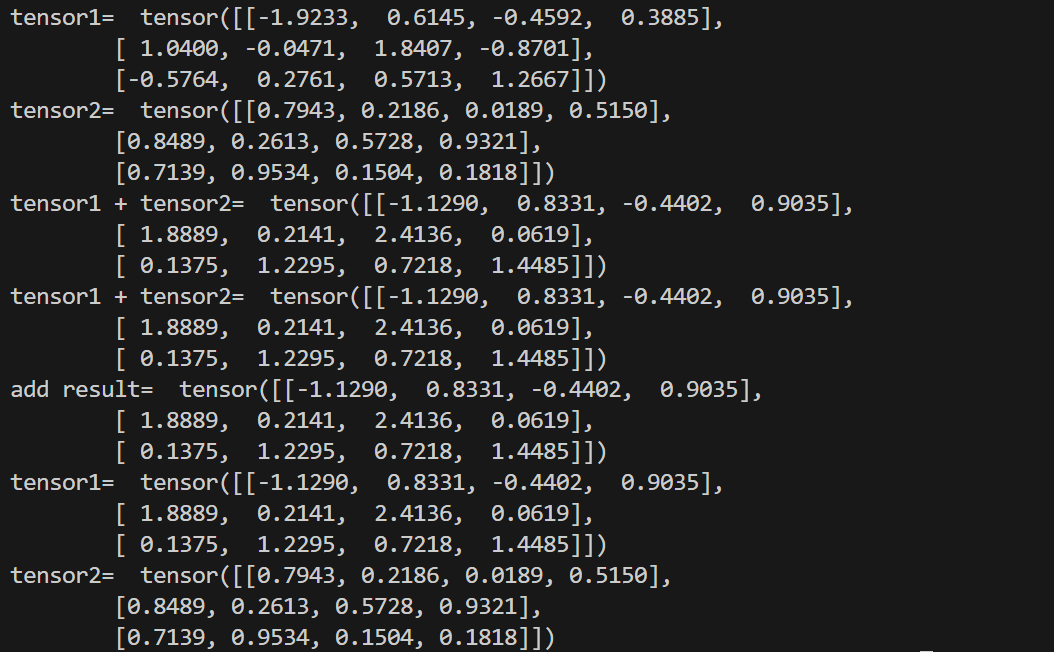
\includegraphics[width=1\textwidth]{./pictures/加法.png}

\subsection{Tensor 转换为 Numpy 数组}
\begin{lstlisting}
a = torch.ones(5)
print(a)
b = a.numpy()
print(b)
\end{lstlisting}
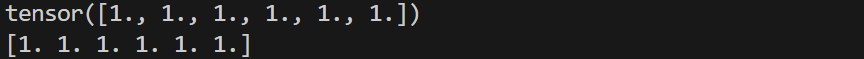
\includegraphics[width=1\textwidth]{./pictures/tensor5.png}
\subsection{Numpy 数组转换为 Tensor}
\begin{lstlisting}
import numpy as np
a = np.ones(5)
b = torch.from_numpy(a)
np.add(a, 1, out=a)
print(a)
print(b)
\end{lstlisting}
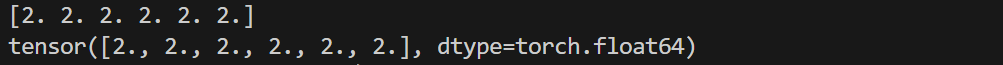
\includegraphics[width=1\textwidth]{./pictures/tensor6.png}
\subsection{CUDA 张量}
\begin{lstlisting}
x = torch.randn(4, 4)

# 当 CUDA 可用的时候,可以使用下方这段代码,采用 torch.device() 方法来改变 tensors 是否在 GPU 上进行计算操作
if torch.cuda.is_available():
    device = torch.device("cuda")          # 定义一个 CUDA 设备对象
    y = torch.ones_like(x, device=device)  # 创建一个在 GPU 上的 tensor
    x = x.to(device)                       # 将 x 移动到 GPU
    z = x + y
    print(z)
    print(z.to("cpu", torch.double))       # 将 z 移动到 CPU 并改变数值类型
else:
    print("CUDA is not available")
\end{lstlisting}
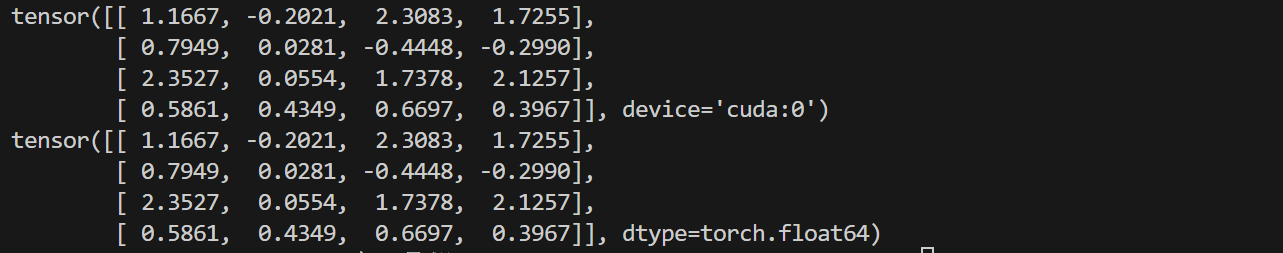
\includegraphics[width=1\textwidth]{./pictures/tensor7.png}
第一个结果是在gpu上运行的,第二个结果是在cpu上运行的。
\subsection{遇到的问题:}
一直报错,说缺少某dll文件,无法运行pytorch,但可以引入torch库。但打开这个文件夹,里面的确是有这个dll文件的。在网上寻找解决方案,下载了新的dll文件放入文件夹内也依然报错。
也考虑过是环境没配置好,重新下载安装了cuda,配置了python的路径等方法都无效。
网上的各种方案都试了一下,都没用。最后尝试重装pytorch,再次运行后发现居然可以了。\par
可能导致问题的原因:第一次下载的时候看到进度条到\verb|100%|就关闭了,导致东西虽然是下完了,但是配置还没完成。
\section{关于本课的感想}
这门课我认为是除了编程课之外最实用的一门课,虽然它没有教我们什么“硬知识”,也只有0.5学分,但它让我们知道了git、latex的存在,让我们学习了shell、命令行、vim的使用,ipdb的调试等等。
老师上课提点一些相关内容,并让我们自己尝试,完成实验、报告的形式也让我们提高了自学能力、独立思考能力。在发现问题并解决问题后,会产生许多的满足感。
并且在《程序设计基础实践》这门课中,我们小组已经全流程使用git进行协同开发了,在开发中我们也深刻体会到了这些工具的重要性。\\
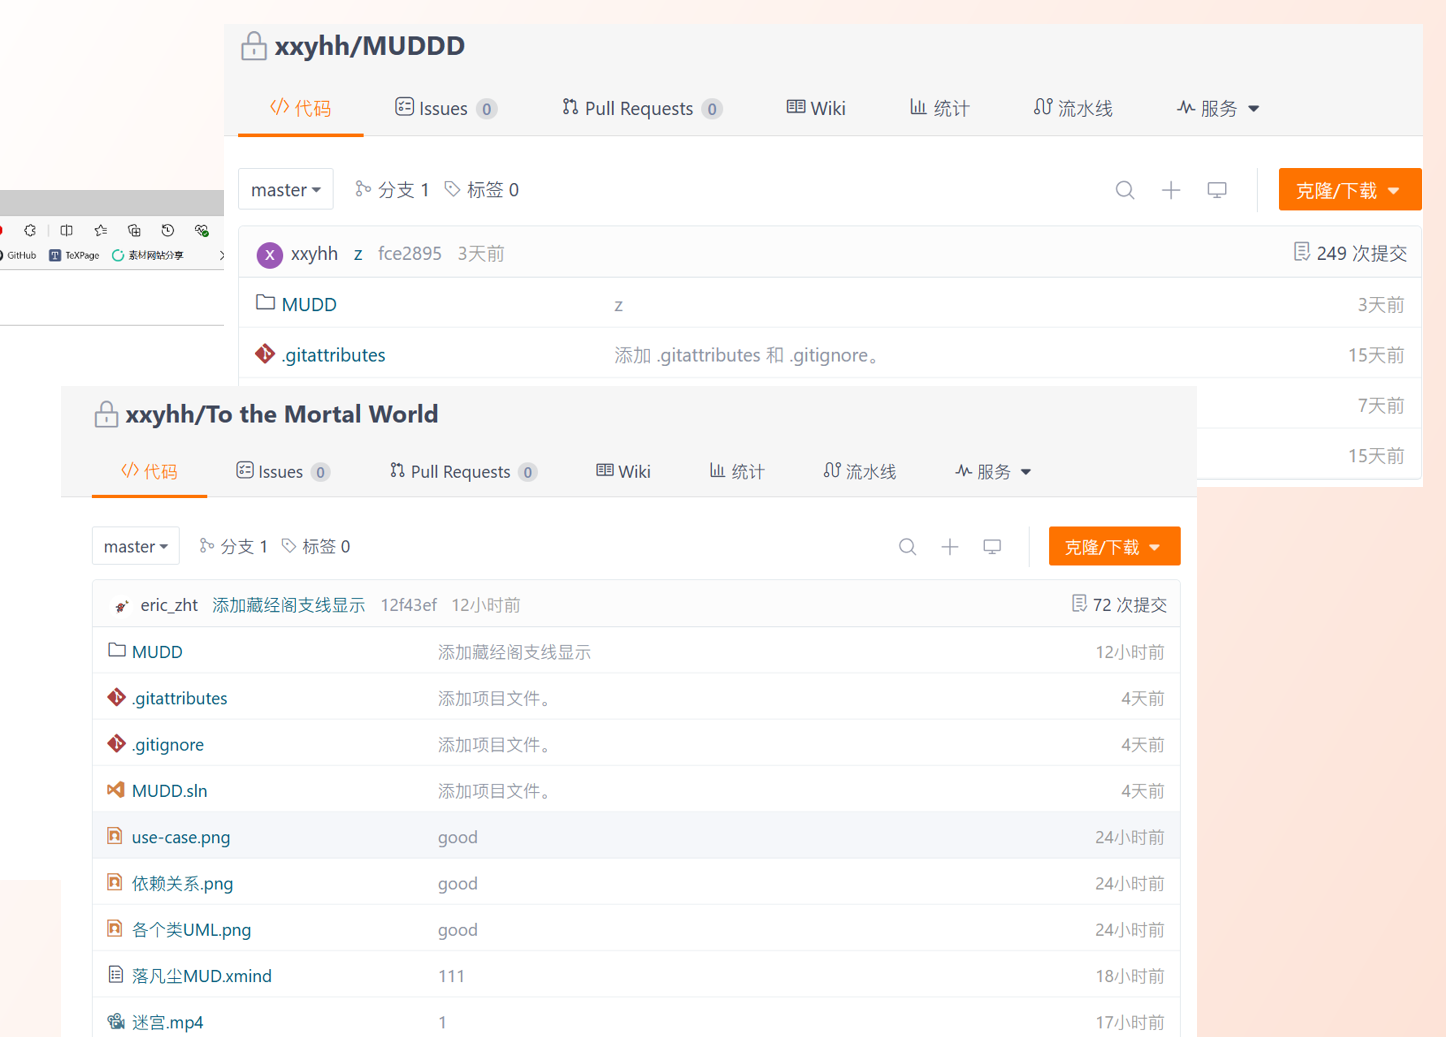
\includegraphics[width=1\textwidth]{./pictures/git.png}
\end{document}
